\chapter{Μέθοδοι προσομοίωσης}
Στο κεφάλαιο αυτό περιγράφεται η υλοποίηση του συστήματος, με βάση τη μελέτη που παρουσιάστηκε στο προηγούμενο κεφάλαιο. 
Αρχικά παρουσιάζεται η πλατφόρμα και τα προγραμματιστικά εργαλεία που χρησιμοποιήθηκαν. 

\section{Εργαλεία που χρησιμοποιήθηκαν}
Για την υλοποίηση των προσομοιώσεων χρησιμοποιήθηκε το πρόγραμμα \en{CST Particle Studio}, της σουίτας προγραμμάτων προσομοίωσης \en{CST Studio Suite}. 
Για την επεξεργασία των αποτελεσμάτων χρησιμοποιήθηκε το πρόγραμμα \en{MATLAB}. 
Τα προγράμματα παρουσιάζονται πιο αναλυτικά παρακάτω.

\subsection{Το \en{CST Particle Studio}}
\begin{figure}[tph]

\includegraphics[width=0.25\textwidth]{images/CST-logo.png}
\centering
\caption{Το λογότυπο του \en{CST}}
\label{img:CSTlogo}
\end{figure}
Το \en{CST PARTICLE STUDIO\textsuperscript{\textregistered} (CST\textsuperscript{\textregistered} PS) } είναι ένα εξειδικευμένο εργαλείο για την γρήγορη και ακριβή ανάλυση δυναμικών φορτισμένων σωματιδίων σε τρισδιάστατα ηλεκτρομαγνητικά πεδία.
Είναι ένα ισχυρό εργαλείο, κατάλληλο για μεγάλο φάσμα εργασιών, από σχεδιασμό \en{magnetrons} και ρύθμιση σωλήνων ηλεκτρονίως έως μοντελοποίηση πηγών σωματιδίων και εξαρτημάτων για επιταχυντές.

%\en{The particle tracking solver can model the behavior of particles through static fields, and with the gun iteration, space charge limited emission. 
Ο \en{particle-in-cell (PIC) solver}, ο οποίος μπορεί να λειτουργήσει στο πεδίο του χρόνου, μπορεί να εκτελέσει μια πλήρη προσομοίωση σωματιδίων και ηλεκτρομαγνητικών πεδίων.

Για σχετικιστικές εφαρμογής, ο \en{wakefield solver} μπορεί να υπολογίσει πώς τα πεδία που δημιουργούνται από σωματίδια που κινούνται στην (ή κοντά στην) ταχύτητα του φωτός, αλληλεπιδρούν με τη δομή γύρω τους.

Το \en{CST PS} έχει ενσωματωμένα τα \en{3D EM modules} του \en{CST STUDIO SUITE\textsuperscript{\textregistered}}, όπως τα \en{CST EM STUDIO\textsuperscript{\textregistered} electro- and magnetostatic solvers} και το \en{CST MICROWAVE STUDIO\textsuperscript{\textregistered} eigenmode solver}.

Είναι πλήρως ενσωματωμένα στο περιβάλλον σχεδίασης \en{CST STUDIO SUITE}, χρησιμοποιώντας έτσι τις δυνατότητες μοντελοποίησης και τα \en{import interfaces}.

Το \en{CST PS} βασίζεται στη γνώση, την έρευνα και την ανάπτυξη των αλγορίθμων που χρησιμοποιήθηκαν στο πακέτο προσομοίωσης \en{MAFIA-4}. 
Ο \en{PIC solver} μπορεί επίσης να εκμεταλλευτεί δυνατότητες \en{GPU computing}, προσφέροντας σημαντικές βελτιώσεις στην απόδοση, σε συμβατό υλικό.

\subsection{Το \en{MATLAB}}
Το \en{MATLAB (matrix laboratory)} είναι ένα περιβάλλον αριθμητικής υπολογιστικής και μια προγραμματιστική γλώσσα τέταρτης γενιάς. 
\en{A proprietary programming language developed by MathWorks, MATLAB allows matrix manipulations, plotting of functions and data, implementation of algorithms, creation of user interfaces, and interfacing with programs written in other languages, including C, C\nolinebreak\hspace{-.05em}\raisebox{.4ex}{\tiny\bf +}\nolinebreak\hspace{-.10em}\raisebox{.4ex}{\tiny\bf +}, C$\sharp$, Java, Fortran and Python.}

\en{Although MATLAB is intended primarily for numerical computing, an optional toolbox uses the MuPAD symbolic engine, allowing access to symbolic computing abilities. 
An additional package, Simulink, adds graphical multi-domain simulation and model-based design for dynamic and embedded systems.}

\begin{figure}[tph]
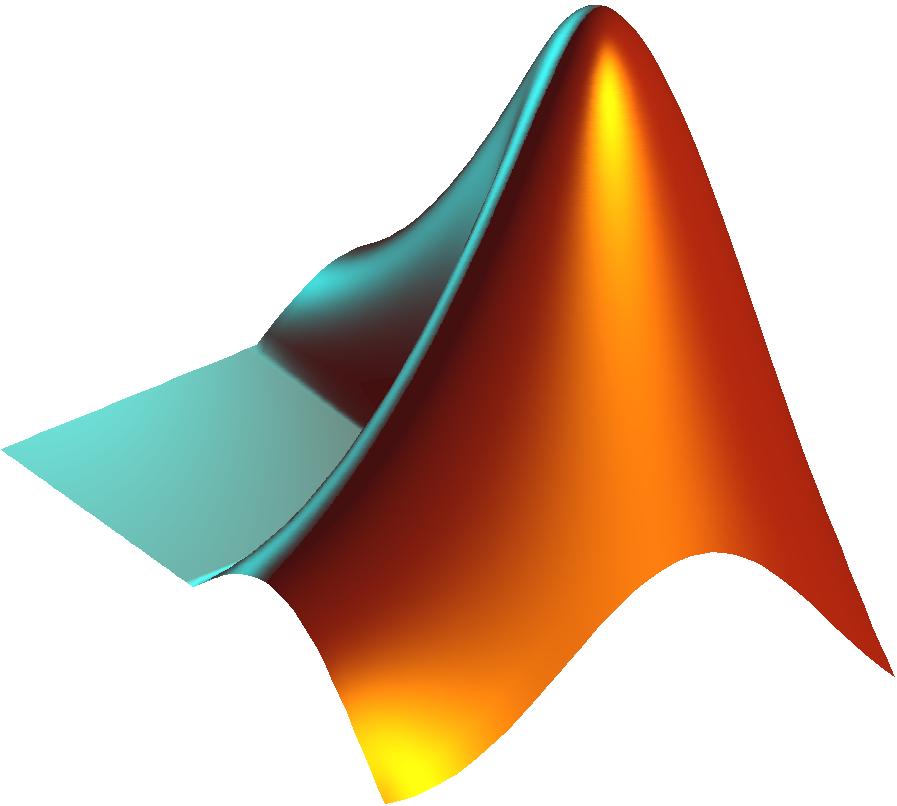
\includegraphics[width=0.25\textwidth]{images/Matlab-logo.png}
\centering
\caption{Το λογότυπο του \en{MATLAB}}
\label{img:MATLABlogo}
\end{figure}

\section{Επιρροή διάφορων μεταβλητών σε έναν \en{Electron Beam Scanner}}
\subsection{Θεωρητική βάση}
Η λεπτή δέσμη ανίχνευσης κινείται κατά τον άξονα $X$, είναι κάθετη στην κίνηση της σχετικιστικής κίνησης της κύριας δέσμης (άξονας $Z$), με παράμετρο απόκλισης $\rho$ (Σχήμα \ref{fig:ellipse-EBS}).

\begin{figure}[tph]
	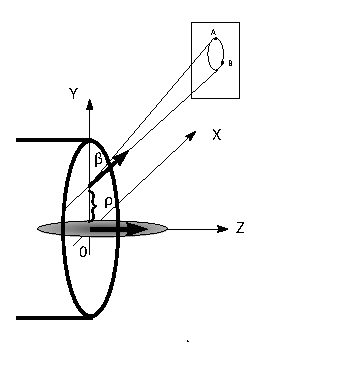
\includegraphics{figures/Logatchov1999-EBS}
	\centering
	\caption{Διαδικασία ανίχνευσης της χαρακτηριστικής έλλειψης της δέσμης}
	\label{fig:ellipse-EBS}
\end{figure}

Τα αποτελέσματα της σάρωσης γίνονται \en{monitor} σε οθόνη παράλληλη στο επίπεδο $Y-Z$ και σε απόσταση $L$ από τον άξονα $Z$.

Έστω ότι το κέντρο της κύριας δέσμης βρίσκεται στην αρχή των αξόνων τη χρονική στιγμή $t = 0$, ενώ η δέσμη ανίχνευσης έχει ομοιόμορφη πυκνότητα κατά $X$ και διάμετρο $d \ll \rho$.
Εδώ υποθέτουμε ότι το $\rho$ είναι μεγαλύτερο του τυπικού εγκάρσιου μεγέθους της κύριας δέσμης.
Τη χρονική στιγμή $t = 0$ κάθε  σωματίδιο της δέσμης ανίχνευσης αντιστοιχίζεται σε μια συγκεκριμένη θέση $x$.
Η συνολική γωνία απόκλισης κατά $Y$ για κάθε σωματίδιο υπό την επιρροή του ηλεκτρικού πεδίου της κύριας δέσμης μπορεί να εκφραστεί ως\cite{Logatchov1999}:
\begin{equation}
\theta_y (x) = \frac{2 \rho r_e}{\beta} \int_{-\infty}^{\infty}\frac{n(z) \dd z}{\rho^2 + \left(x+\beta z \right) ^2}
\end{equation}
όπου:
\begin{itemize}
\item $r_e$: η κλασσική ακτίνα του ηλεκτρονίου,
\item $\beta =\frac{v_t}{c}$: η σχετική ταχύτητα της δέσμης ανίχνευσης,
\item $c$: η ταχύτητα του φωτός,
\item $x$: η θέση σωματιδίου της δέσμης ανίχνευσης τη χρονική στιμή $t=0$,
\item $n(z)$: η γραμμική πυκνότητα της κύριας δέσμης κατά τον άξονα $Z$.
\end{itemize} 

Η έκφραση για τη γωνία απόκλισης του σωματιδίου κατά $Z$, λόγω του μαγνητικού πεδίου, μπορεί να γραφεί\cite{Logatchov1999}:
\begin{equation}
\theta_z(x) = 2 r_e \int_{-\infty}^{\infty}\frac{(x+\beta z)n(z) \dd z}{\rho^2 + \left(x+\beta z \right) ^2}
\end{equation}
\subsection{Αποτελέσματα ανάλυσης με το \en{MATLAB}}
Ιδιαίτερο ενδιαφέρον για την έναρξη της ανάλυσής μας παρουσιάζει το πώς διάφορες μεταβλητές επηρεάζουν τα στοιχεία της χαρακτηριστικής έλλειψης. 
Συγκεκριμένα, θα διερευνήσουμε πώς επηρεάζουν τη χαρακτηριστική έλλειψη οι:
\begin{enumerate}
	\item Ένταση της δέσμης ανίχνευσης
	\item Μήκος της δέσμης ανίχνευσης
	\item Αρχική θέση ριπής κατά $Y$ ($\rho$) 
	\item Τάση της δέσμης ανίχνευσης
\end{enumerate}

Για τη διερεύνηση αυτή δημιουργήθηκε ένα \en{script} στο \en{MATLAB}, όπου χρησιμοποιήθηκε το μοντέλο που παρουσιάστηκε προηγουμένως και έγιναν οι μελέτες για το πώς επηρεάζει η κάθε παράμετρος ξεχωριστά. 
Τα αποτελέσματα φαίνονται παρακάτω.

\begin{figure}[tph]	
	\begin{subfigure}{0.45\textwidth}
		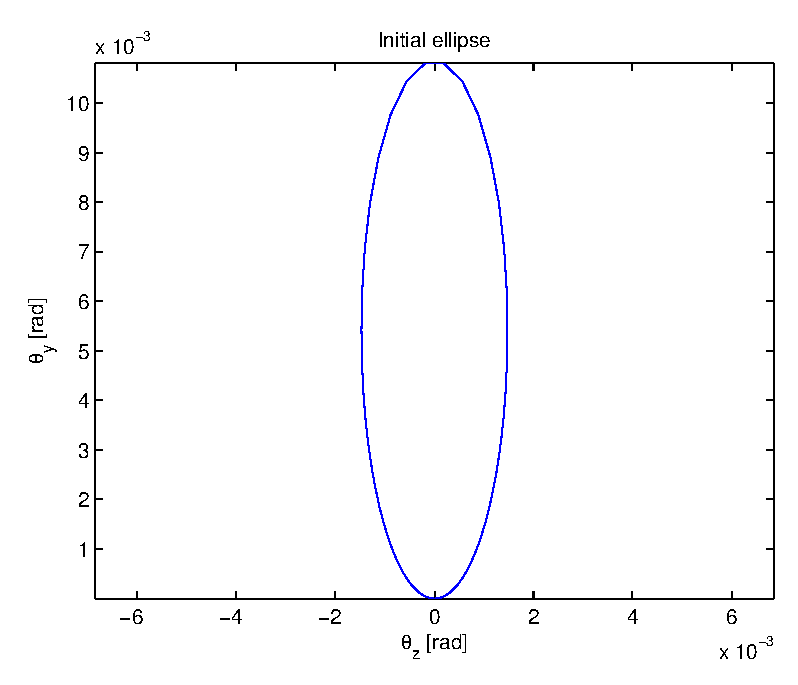
\includegraphics[width=0.9\linewidth]{figures/beam-deflection-script-01-initial-elipse}
		\centering
		\caption{Η χαρακτηριστική έλλειψη στην αρχική κατάσταση}
		\label{fig:beam-deflection-script-01-initial-elipse}
	\end{subfigure}
	~
	\begin{subfigure}{0.45\textwidth}
		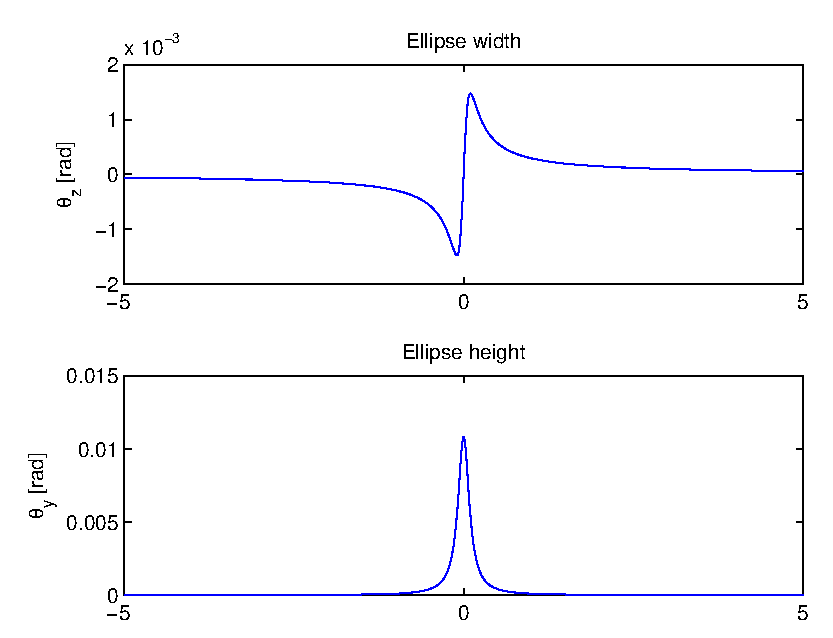
\includegraphics[width=0.9\linewidth]{figures/beam-deflection-script-02-elipse-width}
		\centering
		\caption{Το πλάτος και ύψος της έλλειψης στην αρχική κατάσταση}
		\label{fig:beam-deflection-script-02-elipse-width}
	\end{subfigure}
\caption{Απεικόνιση και στοιχεία της χαρακτηριστικής έλλειψης στην αρχική κατάσταση}
\label{fig:initial-ellipse}
\end{figure}

\begin{figure}[tph]	
	\begin{subfigure}{0.45\textwidth}
		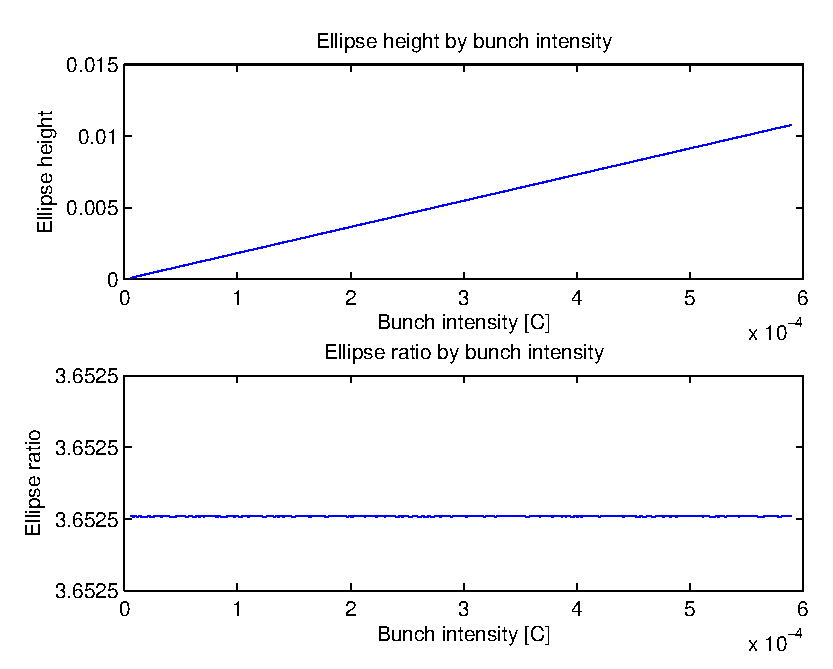
\includegraphics[width=0.9\linewidth]{figures/beam-deflection-script-03-elipse-height}
		\centering
		\caption{Επιρροή της έντασης της δέσμης ανίχνευσης στην ύψος και το λόγο της έλλειψης}
		\label{fig:beam-deflection-script-03-elipse-height}
	\end{subfigure}
	~
	\begin{subfigure}{0.45\textwidth}
		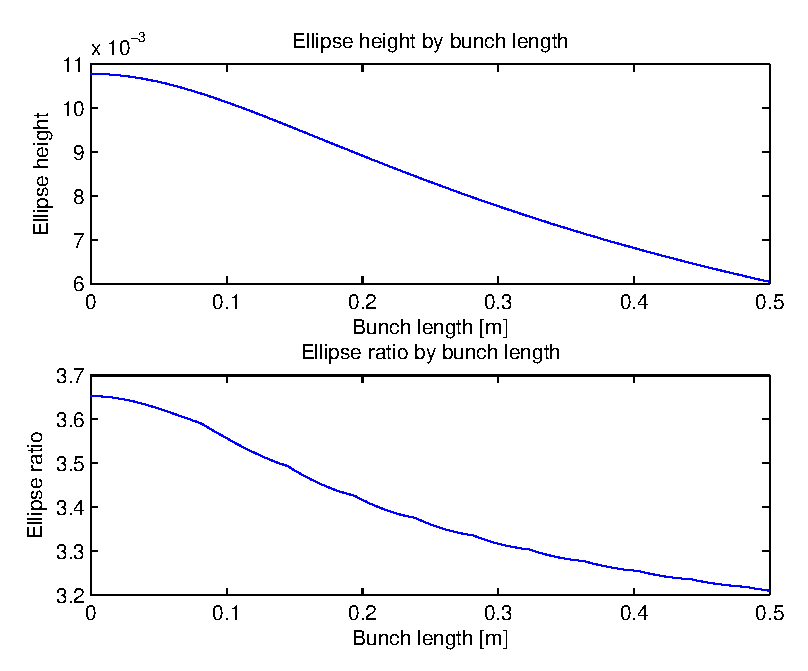
\includegraphics[width=0.9\linewidth]{figures/beam-deflection-script-04-elipse-height-by-bunch-intensity}
		\centering
		\caption{Επιρροή του μήκους της δέσμης ανίχνευσης στην ύψος και το λόγο της έλλειψης}
		\label{fig:beam-deflection-script-04-elipse-height-by-bunch-intensity}
	\end{subfigure}
	\par\bigskip
	\begin{subfigure}{0.45\textwidth}
		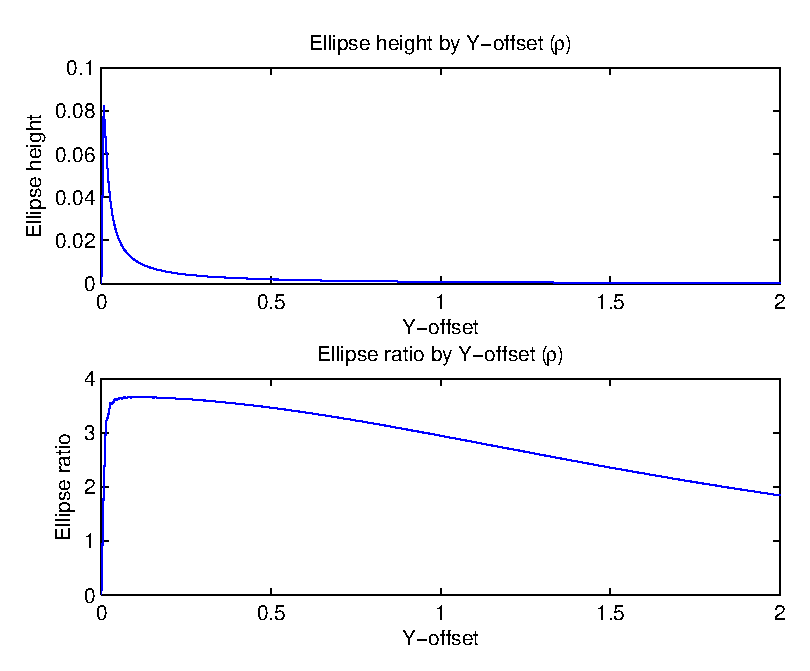
\includegraphics[width=0.9\linewidth]{figures/beam-deflection-script-05-elipse-ratio-by-bunch-intensity}
		\centering
		\caption[Επιρροή της αρχικής θέσης ριπής της δέσμης ανίχνευσης στην ύψος και το λόγο της έλλειψης]{Επιρροή της αρχικής θέσης ριπής ($Y$-\en{offset}) της δέσμης ανίχνευσης στην ύψος και το λόγο της έλλειψης}
		\label{fig:beam-deflection-script-05-elipse-ratio-by-bunch-intensity}
	\end{subfigure}
	~
	\begin{subfigure}{0.45\textwidth}
		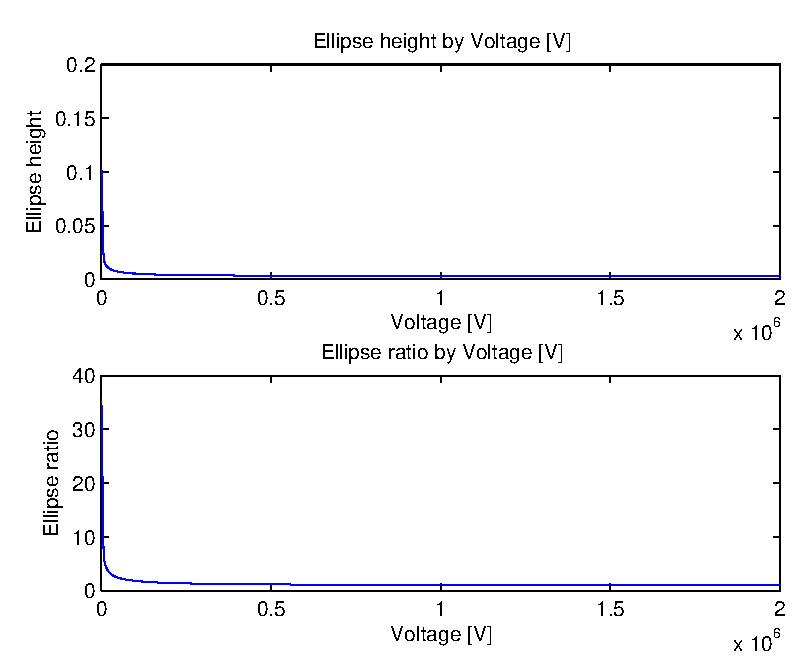
\includegraphics[width=0.9\linewidth]{figures/beam-deflection-script-06}
		\centering
		\caption{Επιρροή της γραμμικής μεταβολής τάσης της δέσμης ανίχνευσης στην ύψος και το λόγο της έλλειψης}
		\label{fig:beam-deflection-script-06}
	\end{subfigure}
	\par\bigskip
	\begin{subfigure}{0.45\textwidth}
		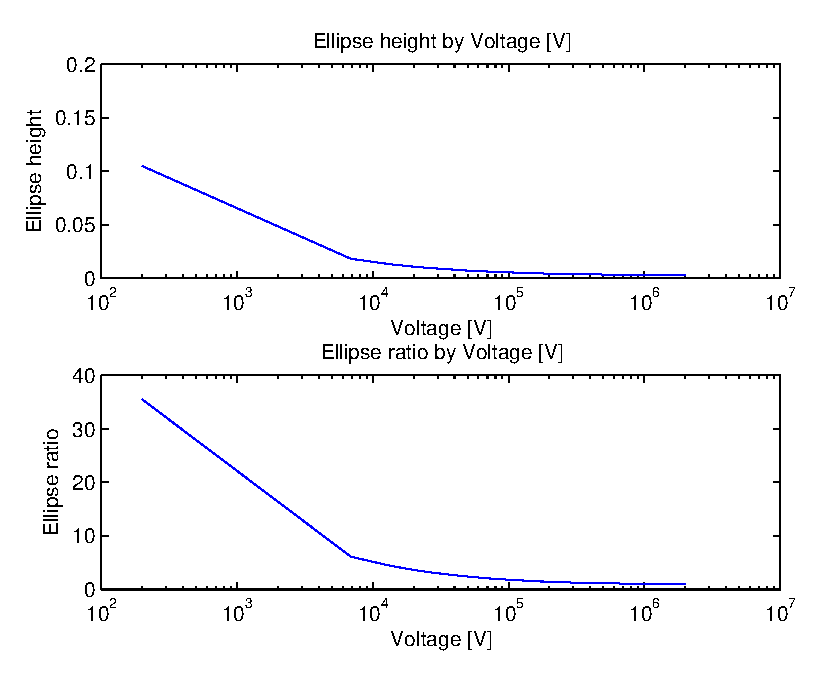
\includegraphics[width=0.9\linewidth]{figures/beam-deflection-script-07}
		\centering
		\caption{Επιρροή της εκθετικής μεταβολής τάσης της δέσμης ανίχνευσης στην ύψος και το λόγο της έλλειψης}
		\label{fig:beam-deflection-script-07}
	\end{subfigure}
\caption{Επιρροή διαφόρων μεγεθών στη χαρακτηριστική έλλειψη}
\label{fig:beam-deflectoin}
\end{figure}

\subsection{Αποτελέσματα ανάλυσης με το \en{CST}}

Στη συνέχεια έγινε η ίδια ανάλυση στο περιβάλλον προσομοίωσης του \en{CST} για την επαλήθευση των αποτελεσμάτων. 
Για να γίνει αυτό αρχικά δημιουργήθηκε το περιβάλλον προσομοίωσης, και σε αυτό μπήκαν οι  δυο κύλινδροι, μέσα στους οποίους βρίσκονται οι 2 δέσμες, η κύρια δέσμη και η δέσμη ανίχνευσης (Σχήμα \ref{fig:CST-PICmonitor}). 
Στη συνέχεια προστέθηκαν οι πηγές σωματιδίων ως κυκλικές πηγές, με την κύρια πηγή να έχει \en{Gaussian} προφίλ, ενώ η πηγή της δέσμης ανίχνευσης σταθερό. 
Η πηγή σωματιδίων της κύριας δέσμης φαίνεται στο Σχήμα \ref{fig:CST-mainBeamSource}.

\begin{figure}[tbh]
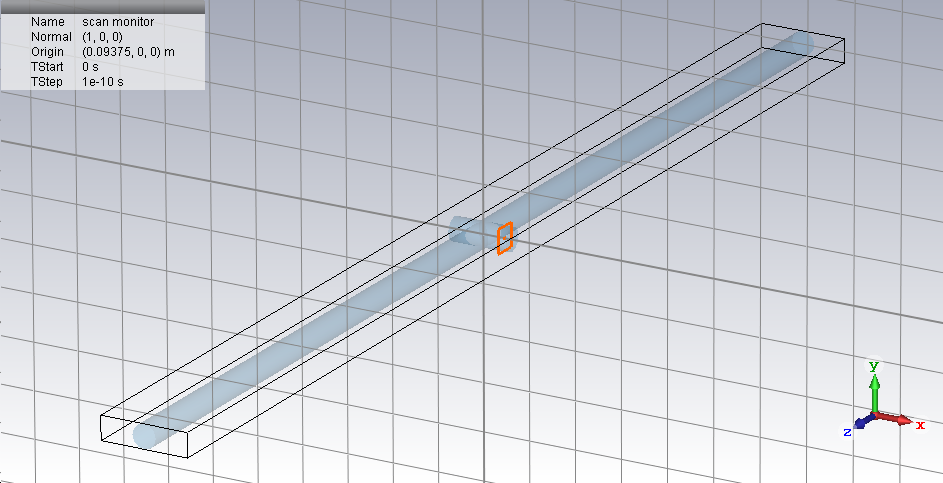
\includegraphics[width=\textwidth]{figures/CST-pic-monitor}
\centering
\caption[Η διάταξη προσομοιωμένη στο \en{CST}]{Η διάταξη προσομοιωμένη στο \en{CST}. 
Στην κύρια δέσμη φαίνεται ανιχνευτής σωματιδίων λίγο πριν το σημείο που γίνεται η ανίχνευση}
\label{fig:CST-PICmonitor}
\end{figure}

\begin{figure}[tbh]
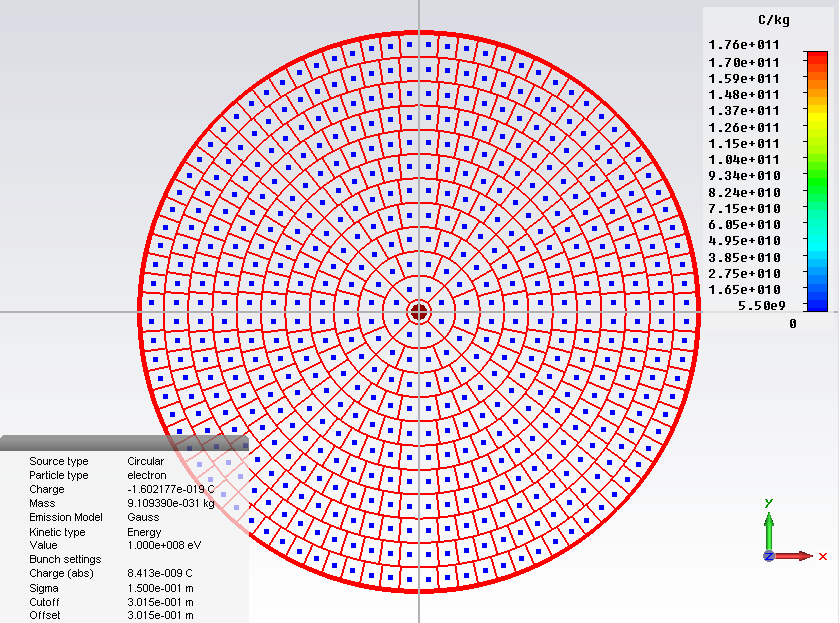
\includegraphics[width=0.5\textwidth]{figures/CST-main-beam-source}
\centering
\caption{Η πηγή της κύριας δέσμης στο \en{CST}}
\label{fig:CST-mainBeamSource}
\end{figure}

Τα αποτελέσματα της προσομοίωσης σε φαίνονται παρακάτω. 

%TODO create and add images of the simulation (file 0.21?)

\section{Εκτίμηση του προφίλ στατικής δέσμης στο \en{CST}}

Αφού είδαμε ότι είναι εφικτό να μετρηθούν τα χαρακτηριστικά με τον τρόπο που προσομοιώνει το \en{CST}, ως επόμενο βήμα θα υπολογίσουμε το ακριβές προφίλ της δέσμης, δηλαδή θα δημιουργήσουμε έναν \en{Electron Beam Scanner}.

\begin{figure}[tph]
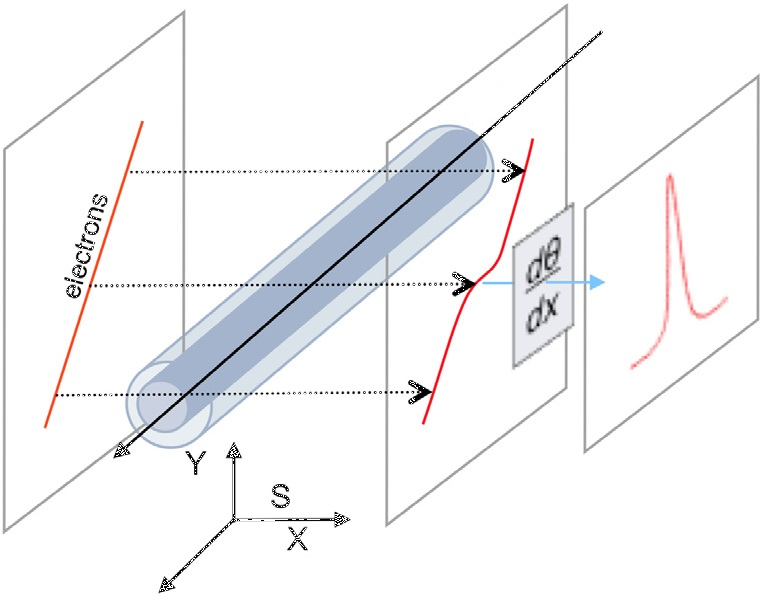
\includegraphics[width=0.5\textwidth]{figures/EBS-profile-calculation}
\centering
\caption{Υπολογισμός του προφίλ δέσμης με \en{Electron Beam Scanner}}
\label{fig:EBS-profile-calculation}
\end{figure}

Όπως είδαμε και στο προηγούμενο κεφάλαιο, το προφίλ της δέσμης προκύπτει από την παραγώγιση  της απόκλισης $\theta_y$.

Στην περίπτωσή μας, ο υπολογισμός τους προφίλ γίνεται μέσα στο \en{CST}, στο στάδιο του \en{post-processing}.



\section{Εκτίμηση του προφίλ \en{Gaussian} δέσμης στο \en{CST}}

Για τον υπολογισμό του προφίλ μιας \en{Gaussian} δέσμης, συναντήσαμε το πρόβλημα ότι μετά τον υπολογισμό του προφίλ, το σχήμα δε φαινόταν να έχει αυτό που ήταν αναμενόμενο.

\begin{figure}[tph]
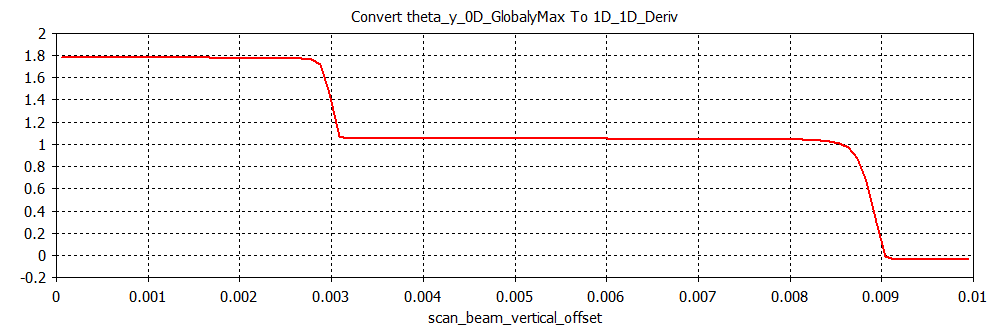
\includegraphics[width=\textwidth]{figures/CST-profile-steps}
\centering
\caption{Το αποτέλεσμα του υπολογισμού του προφίλ στο \en{CST} δε μοιάζει \en{Gaussian}}
\label{fig:CST-profile-steps}
\end{figure}

Για την επίλυση του προβλήματος αυτού, αρχικά ελέγξαμε αν το πρόβλημα βρίσκεται στον τρόπο δημιουργίας της δέσμης ή στον τρόπο ανίχνευσης. 
Έτσι:
\begin{enumerate}
\item Δημιουργήσαμε ένα νέο project και, αφού στήθηκε όλο το μοντέλο εκ νέου, μπήκε ένας \en{particle monitor} που ανιχνεύει τα σωματίδια της κύριας δέσμης
\item Έγινε εξαγωγή των δεδομένων αυτών της κύριας δέσμης
\item Τα δεδομένα αυτά εισήχθησαν στο \en{MATLAB} και δημιουργήθηκε το κατάλληλο \en{script} για την ανάλυσή τους
\end{enumerate}

Από την παραπάνω διαδικασία έγινε σαφές ότι το πρόβλημα εντοπίζεται στον τρόπο που το \en{CST} δημιουργεί την κατανομή των σωματιδίων.

\subsection{Τρόπος δημιουργίας \en{Gaussian} κατανομών σωματιδίων στο \en{CST}}

Μετά από αναζήτηση και επικοινωνία με το ίδιο το \en{support} του \en{CST}, έγινε σαφής ο τρόπος που γίνεται η προσομοίωση των σωματιδίων για \en{Gaussian} κυκλικές πηγές σωματιδίων.
%TODO citation needed
Συγκεκριμένα, αρχικά, αφού το συνολικό ποσό φορτίου που εκπέμπεται δεν μεταβάλλεται ανάλογα με τη συνάρτηση κατανομής τίθεται ο περιορισμός ότι:
\begin{equation}\label{eq:CST-gaussian-restriction}
2\pi \int_{R_{in}}^{R_{out}} f(r) \dd r = \pi \left(R_{out}^2 - R_{in}^2 \right) 
\end{equation}

όπου:
\begin{itemize}
\item $R_{out}$: η εξωτερική ακτίνα της κυκλικής πηγής σωματιδίων
\item $R_{in}$: η εσωτερική ακτίνα της κυκλικής πηγής σωματιδίων (στην περίπτωσή μας $R_{in} = 0$)
\item $f(r)$: η συνάρτηση ακτινικής κατανομής 
\end{itemize} 

Η παραπάνω σχέση χρησιμοποιείται για να κλιμακοποιήσει τη συνάρτηση κατανομής. 
Αυτό σημαίνει ότι ο συντελεστής κατανομής $c_{scale}$ υπολογίζεται αυτόματα.

Στη συνέχεια, η \en{Gaussian} κατανομή δίνεται από τη σχέση:
\begin{equation}
f(r) = c_{off} + c_{scale} \left( \exp \left(-\frac{r^2}{2\sigma^2}\right) - 1 \right)
\end{equation}

όπου:
\begin{itemize}
\item $c_{off}$: η τιμή της συνάρτησης για $r = 0$
\item $\sigma$: η τυπική απόκλιση
\end{itemize} 

\begin{figure}[tph]
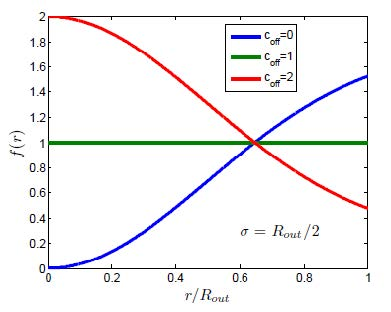
\includegraphics{figures/CST-gauss-function-for-coff}
\centering
\caption{Παράδειγμα \en{Gaussian} συνάρτησης για διάφορες τιμές του συντελεστή $c_{off}$}
\label{fig:CST-gauss-coff}
\end{figure}

Για να έχουμε μια πραγματικά \en{Gaussian} δέσμη, θέλουμε να ισχύει
\[c_{off} = 0\]

Αφού οι υπόλοιπες μεταβλητές είναι καθορισμένες από τις απαιτήσεις του επιταχυντή, απομένει να βρεθεί η τιμή του $c_{scale}$ που θα μας δίνει τη ζητούμενη συνθήκη.

\subsection{Υπολογισμός του κατάλληλου συντελεστή κλιμακοποίησης για \en{Gaussian} δέσμη}

Ο τρόπος που υπολογίζει το \en{CST} την \en{Gaussian} κατανομή, όπως είδαμε παραπάνω είναι
\begin{eqnarray}\label{eq:CST-gaussian-model}
f(r) &= & 	c_{off} + c_{scale} \left( \exp \left(-\frac{r^2}{2\sigma^2}\right) - 1 \right) \nonumber \\
&= &\left(c_{off} - c_{scale}\right) + c_{scale} e^{-\frac{r^2}{2\sigma^2}}
\end{eqnarray}

Η πραγματική κατανομή της δέσμης στον επιταχυντή που μελετούμε όμως, έχει γενική μορφή κατανομής:
\begin{equation}\label{eq:General-gaussian-model}
 f(r) = a e^{-\frac{\left(r-b\right)^2}{2c^2}}
\end{equation}

Επομένως, εξισώνοντας τις παραπάνω σχέσεις \ref{eq:CST-gaussian-model} και \ref{eq:General-gaussian-model} και δεδομένου ότι πρέπει να ισχύουν $\forall r$ προκύπτουν τα συμπεράσματα ότι:
\begin{eqnarray}
a &\equiv & c_{scale}\nonumber \\
b &\equiv &0\nonumber \\
c &\equiv & \sigma \nonumber \\
c_{off} &=&  c_{scale} 
\end{eqnarray}

Επομένως, πρέπει να βρεθεί ο κατάλληλος συνδυασμός τιμών $\left(c_{off}, c_{scale}\right)$ που να πληροί τον περιορισμό της εξίσωσης \ref{eq:CST-gaussian-restriction}, δεδομένων των τιμών των μεταβλητών $\sigma, R_{out}$ και $R_{in}$ του επιταχυντή μας.

Για την επίλυση του παραπάνω προβλήματος δημιουργήθηκε κατάλληλο \en{script} στο \en{MATLAB}. 

Αρχικά δημιουργήθηκε η συνάρτηση \src{cscale = calculateCscale( sigma, coff, Rout, Rin)} η οποία δέχεται ως ορίσματα τις μεταβλητές $\sigma, c_{off}, R_{out}$ και $R_{in}$ και δίνει στην έξοδό του την τιμή του $c_{scale}$ που πληροί την εξίσωση \ref{eq:CST-gaussian-restriction}.

Στη συνέχεια, τρέχοντας το \en{script} \src{findOptimumCoff.m} δίνουμε τις τιμές των παραμέτρων του προβλήματός μας στα $\sigma, c_{off}, R_{out}, R_{in}$ και βρίσκουμε την τιμή του $c_{off}$ που επαληθεύει τη σχέση $c_{off} = c_{scale} \left(\sigma, c_{off}, R_{out}, R_{in} \right)$.

\lstinputlisting[caption={\tg{Η συνάρτηση υπολογισμού του $c_{scale}$}}]{code/Calculating-optimum-coff/calculateCscale.m}
\lstinputlisting[caption={\tg{Το }\en{script}\tg{ υπολογισμού του κατάλληλου για τα δεδομένα μας $c_{off}$}}]{code/Calculating-optimum-coff/findOptimumCoff.m}
%TODO fix this shit

Εν τέλει, για τις τιμές του δικού μας προβλήματος, δίνουμε ως είσοδο $\left(\sigma, R_{out}, R_{in} \right) = \left(0.01/4,0.01, 0 \right)$ και προκύπτει ότι:
\begin{equation}
c_{off} \approx 8.002684
\end{equation}

\section{Επιρροή αλλεπάλληλων δεσμών στο προφίλ δέσμης}

\section{Επαλήθευση αποτελεσμάτων στο \en{MATLAB}}

